\documentclass[msc]{thesis}
%\documentclass[msc]{thesis}

\authorfirstname{Firstname}
\authorlastname{Lastname}

\reviewer{Gutachter}{
    \referentname{Prof.~Dr.~Martin Butz}\\
    \referentinstitute{
        Kognitive Modellierung\\
        Wilhelm-Schickard-Institut für Informatik\\
        Universität Tübingen
    }\\
	[0.3cm]
    \referentname{Prof.~Dr.~Nitram Ztub}\\
    \referentinstitute{
        Kognitive Modellierung\\
        Wilhelm-Schickard-Institut für Informatik\\
        Universität Tübingen
    }
}

% optional
\supervisor{Betreuer}{
    \referentname{Dr.~Vorname Nachname}\\
    \referentinstitute{
        Kognitive Modellierung\\
        Wilhelm-Schickard-Institut für Informatik\\
        Universität Tübingen
    }
}


\course{Kognitionswissenschaft}
%\course{Informatik}
%\course{Weltrauminformatik

\title{This is a Fancy Topic}
\date{\today}
\editingperiod{01.01.2019 -- 01.04.2019}

\setlength\cftbeforechapskip{2pt}

\makeatletter

%%%%%%%%%%%%%%%%%%%%%%%%
\hypersetup{
    bookmarksopen={true},
    bookmarksopenlevel={0},
    bookmarksnumbered={true},
    breaklinks={true},
    colorlinks={false},
    pdfpagemode={UseOutlines},
    pdftitle={\@title},
    pdfauthor={\@author},
    pdfsubject={\thethesistype},
    pdfview={FitV},
    pdffitwindow={true},
    pdfstartview={FitV},
    pdfnewwindow={false},
    pdfdisplaydoctitle={true},
    pdfhighlight={/P},
    plainpages={false},
    unicode={true},
    urlcolor={blue}
}

\makeatother

\begin{document}
\frontmatter

\selectlanguage{ngerman}

\maketitle

\selectlanguage{english}
\chapter*{Abstract}
\markboth{Abstract}{Abstract}
...


\selectlanguage{ngerman}
\chapter*{Kurzfassung}
\markboth{Kurzfassung}{Kurzfassung}



\selectlanguage{english}

\tableofcontents


\mainmatter

\selectlanguage{english}

%----------------------------------------------------------------
% Content
%----------------------------------------------------------------

\chapter{Introduction}\label{chapter:introduction}
%
Human vision is inherently selective. Rather than processing the entire visual field uniformly, 
the human eye relies on a foveated view, where high-resolution vision is concentrated in a small central region (the fovea), 
while the surrounding peripheral vision is of lower resolution.
Humans sequentially direct their gaze towards interesting or task-relevant regions of a scene,
integrating information over time to form a coherent understanding of their environment.
This mechanism of selective attention allows humans to efficiently process complex visual scenes under limited computational resources.\\\\
%
In contrast, most artificial vision systems process visual inputs in a uniform manner,
requiring high computational resources to achieve comparable performance to human vision.
They also usually only use a single feedforward pass to process an image, leading to limited interpretability and adaptability to changing environments.\\\\
%
Research in active vision and attention-based reinforcement learning has begun to address these limitations.
Models such as the Recurrent Attention Model (RAM) \citep{mnih2014recurrentmodelsvisualattention} and its variants have demonstrated
the potential of foveated vision and sequential attention mechanisms in artificial agents.


\chapter{Foundations}\label{chapter:foundations}
%



\begin{figure}[t]
    \centering
    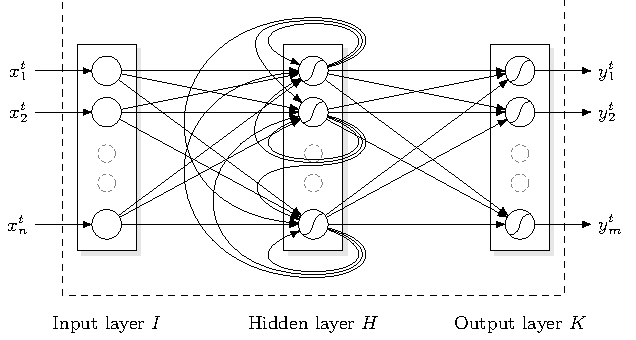
\includegraphics[]{figures/rnnfull/rnnfull}
    \caption{Lorem ipsum dolor sit amet, consetetur sadipscing elitr, sed diam nonumy eirmod tempor invidunt ut labore et dolore magna aliquyam erat, sed diam voluptua. At vero eos et accusam et justo duo dolores et ea rebum. Stet clita kasd gubergren, no sea takimata sanctus est Lorem ipsum dolor sit amet.}
    \label{figure:rnnfull}
\end{figure}



\begin{table}[t]
\centering
\caption{Interesting table}
\label{table:data}
\small
\begin{tabularx}{\textwidth}{XXXX}
\toprule
Column A & Column B & Column C & Column D\\
\midrule
1 & 2 & 3 & 4\\
5 & 6 & 7 & 8\\
9 & 10 & 11 & 12\\
13 & 14 & 15 & 16\\
\bottomrule
\end{tabularx}    
    
    
\end{table}
\chapter{Conclusion and Future Work}\label{chapter:conclusion}
%



%----------------------------------------------------------------
% appendix chapter format
%----------------------------------------------------------------
\appendix

\chapter{Important Additional Stuff}\label{appendix:ias}   

\backmatter

%----------------------------------------------------------------
% abbreviations
%----------------------------------------------------------------

\include{misc/abbreviations}

%----------------------------------------------------------------
% bibliography
%----------------------------------------------------------------

\bibliographystyle{natbib}
\bibliography{thesis}

\cleardoublepage
\thispagestyle{empty}
\section*{Selbständigkeitserklärung}

Hiermit versichere ich, dass ich die vorliegende {\thethesistype} 
selbständig und nur mit den angegebenen Hilfsmitteln angefertigt habe und dass alle Stellen, die dem Wortlaut oder dem 
Sinne nach anderen Werken entnommen sind, durch Angaben von Quellen als 
Entlehnung kenntlich gemacht worden sind. 
Diese {\thethesistype} wurde in gleicher oder ähnlicher Form in keinem anderen Studiengang als Prüfungs\-leistung vorgelegt. 

\vspace{3cm}

\begin{center}
\begin{tabular}{p{0.32\linewidth}p{0.25\linewidth}p{0.32\linewidth}}
\hrule\vspace{0.2cm}
\centering Ort, Datum
& &  
\hrule\vspace{0.2cm}
\centering Unterschrift 
\end{tabular}
\end{center}

\end{document}
